% This file was created by matlab2tikz.
%
%The latest updates can be retrieved from
%  http://www.mathworks.com/matlabcentral/fileexchange/22022-matlab2tikz-matlab2tikz
%where you can also make suggestions and rate matlab2tikz.
%
\definecolor{mycolor1}{rgb}{1.00000,0.20000,0.10000}%
%
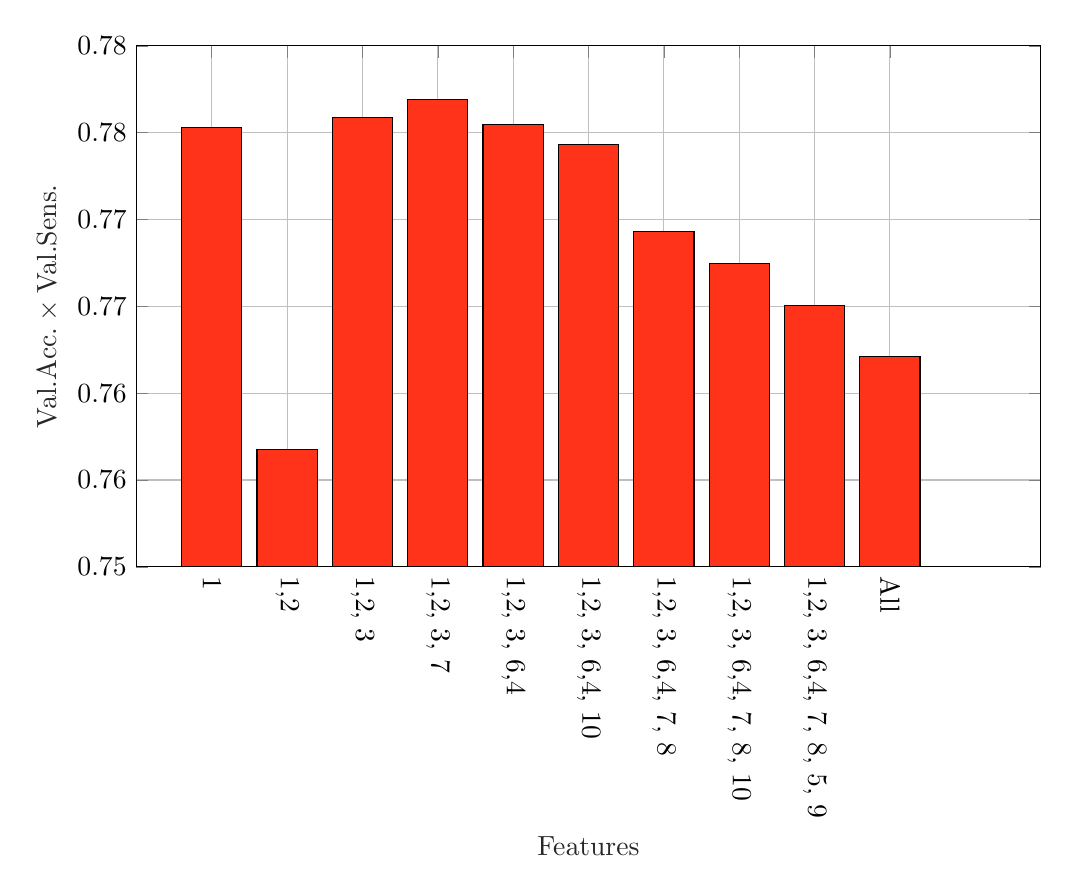
\begin{tikzpicture}

\begin{axis}[%
width=4.521in,
height=2.605in,
at={(0.758in,1.442in)},
scale only axis,
bar shift auto,
log origin=infty,
xmin=0,
xmax=12,
xtick={1,2,3,4,5,6,7,8,9,10},
xticklabels={{1},{1,2},{1,2, 3},{1,2, 3, 7},{1,2, 3, 6,4},{1,2, 3, 6,4, 10},{1,2, 3, 6,4, 7, 8},{1,2, 3, 6,4, 7, 8,  10},{1,2, 3, 6,4, 7, 8,  5,  9},{All}},
xticklabel style={rotate=270},
xlabel style={font=\color{white!15!black}},
xlabel={Features},
ymin=0.75,
ymax=0.78,
ylabel style={font=\color{white!15!black}},
ylabel={$\mathrm{Val. Acc.} \times \mathrm{Val. Sens.}$},
axis background/.style={fill=white},
xmajorgrids,
ymajorgrids
]
\addplot[ybar, bar width=0.8, fill=mycolor1, draw=black, area legend] table[row sep=crcr] {%
1	0.775289941972919\\
2	0.756738394584139\\
3	0.775892649903287\\
4	0.776920889748548\\
5	0.775485783365569\\
6	0.77432572533849\\
7	0.769306092843325\\
8	0.76746324951644\\
9	0.765066150870405\\
10	0.762097872340424\\
};
\end{axis}
\end{tikzpicture}%